\section{Standard deviation}

The initial two analyses conducted can be considered general and applicable universally, as the computed quantities consistently have the same interpretation. Our focus now is to utilize the standard deviation of the predicted distribution, considering it as a categorical distribution where the classes are interpreted as numerical values.

This concept can be formalized by introducing $Y$ as the output variable, capable of assuming integer values within the range $[0,9]$, with probabilities denoted as $p_i$ to assume the value $i$, which are predicted by the network. The expected value of this variable can be computed as follows:

\[
	E[Y] = \sum_{i=0}^{9} i \cdot p_i
\]

Following the definition of variance, we obtain:

\[
	Var[Y] = E[(Y - E[Y])^2] = \sum_{i=0}^{9} (i - E[Y])^2 \cdot p_i = \sigma^2
\]

To obtain the desired metric, we simply take the square root of the variance:

\[
	sd[Y] = \sqrt{Var[Y]} = \sigma
\]

It's important to highlight that this metric diverges from the previous one due to its reliance on the specific domain; for instance, it might not be easily applicable to tasks involving a hundred of classes instead of ten.
In the case analyzed in this thesis, the application is intuitive since the task is to classify digits. However, such intuitive alignment may not be easily transferable to other tasks, such as animal classification.

Following the same procedure of the previous cases we tried to identify a reasonable range for the threshold regarding the standard deviation. This metric allows the determination of an upper and a lower bound:

\begin{itemize}
	\item Case minimum uncertainty: $\hat{p}$ has all terms equal to 0 except one which is 1. This leads to $\sigma=0$.
	\item Case maximum uncertainty: $\hat{p}$ has all values the same. In this case it results $\sigma = 2.87$.
\end{itemize}

The threshold is defined as linear function of the desired confidence level, as the previously:

\[
	threshold = 2.87 * (1 - conf \_ level), \ with \ con \_ level \in [0,1]
\]

The outcomes of this approach are visually illustrated in \Fig~\ref{fig:std_class}. It is possible to note that the accuracy, \Fig~\ref{fig:std_acc}, has a smoother behavior than the previous cases. The maximum accuracy reached is around $99.4\%$, showcasing a marginal improvement over the aleatoric uncertainty. The better behavior can be attributed to the utilization of a more specific domain metric. However, as before, a deeper analysis is necessary to validate its effectiveness.
In \Fig~\ref{fig:std_unk} it is shown the trend of the unknowns values, which increases when the confidence level is increased as expected.
The case $conf_{level}=1$ leads again to a complete loss of the network usefulness.

\begin{figure}[h]
	\centering
	\begin{subfigure}{.5\textwidth}
		\centering
		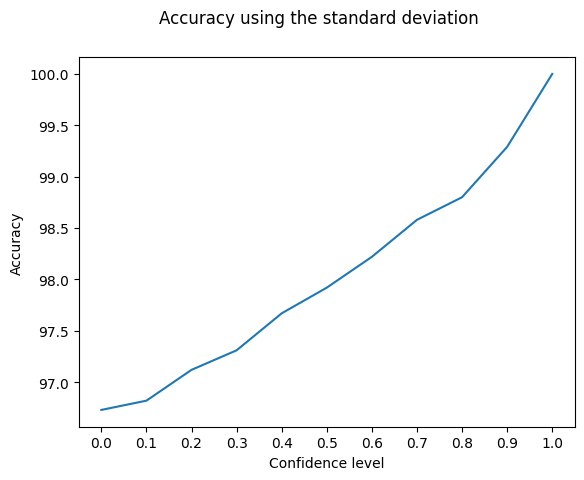
\includegraphics[width=0.8\linewidth]{ImageFiles/ClassifUncer/std_acc}
		\caption{Accuracy trend when the confidence level is increased}
		\label{fig:std_acc}
	\end{subfigure}%
	\begin{subfigure}{.5\textwidth}
		\centering
		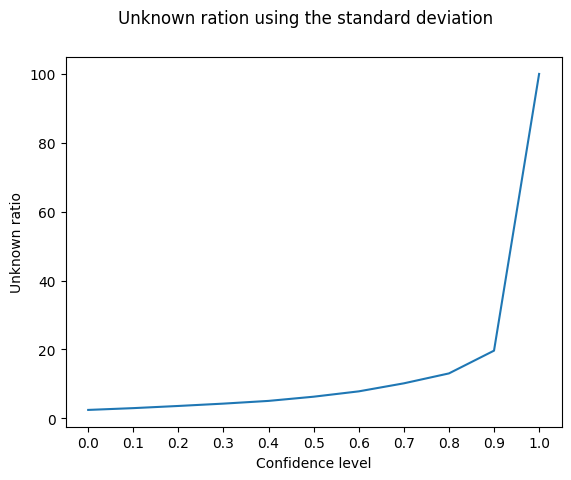
\includegraphics[width=0.8\linewidth]{ImageFiles/ClassifUncer/std_unk}
		\caption{Unknown ratio trend when the confidence level is increased}
		\label{fig:std_unk}
	\end{subfigure}
	\caption{Performances of the BNN using the standard deviation during classification}
	\label{fig:std_class}
\end{figure}